\section{Vision Transformer}

\begin{frame}[fragile]{Mathematical Foundations}
\framesubtitle{TODO}

\end{frame}

\begin{frame}[fragile]{Vision Transformer Architecture}
\framesubtitle{Patch Embedding and Positional Econding}

\end{frame}

\begin{frame}[fragile]{Vision Transformer Architecture}
\framesubtitle{Transformer Encoder and Classification Head}

\end{frame}

\begin{frame}[fragile]{ViT vs. CNN}
  \begin{columns}
    \begin{column}{\textwidth}
      \begin{itemize}
        \item CNNs use convolutional layers with local receptive fields.
        \item ViTs process images globally using self-attention mechanisms.
        \item CNNs have built-in spatial hierarchies, whereas ViTs rely on attention.
        \item ViTs typically need more data to perform well but can model long-range dependencies.
      \end{itemize}
    \end{column}
  \end{columns}
  \begin{figure}
    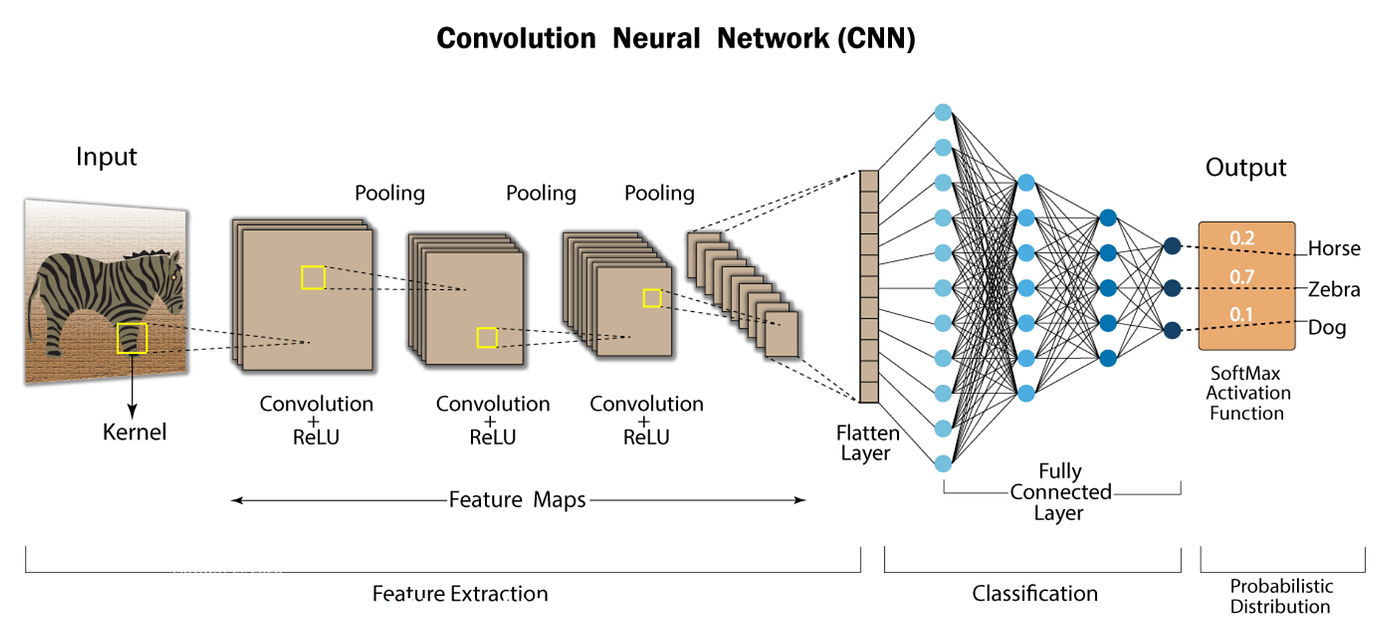
\includegraphics[width=0.6\textwidth]{images/cnn_architecture.png}
  \end{figure}
\end{frame}